\documentclass[landscape,a0paper,fontscale=0.292]{baposter}

\usepackage[vlined]{algorithm2e}
\usepackage{times}
\usepackage{calc}
\usepackage{url}
\usepackage{graphicx}
\usepackage{amsmath}
\usepackage{amssymb}
\usepackage{relsize}
\usepackage{multirow}
\usepackage{booktabs}

\usepackage{graphicx}
\usepackage{multicol}
\usepackage[T1]{fontenc}
\usepackage{ae}
\usepackage{enumitem}

\usepackage{colortbl}
\usepackage{xcolor}
%\usepackage{gensymb} % for \degree
\graphicspath{{figs/}}

\setlist[itemize]{leftmargin=*,nosep}
    \setlength{\columnsep}{0.7em}
    \setlength{\columnseprule}{0mm}

\setlist[enumerate]{leftmargin=2.5em,nosep}
    \setlength{\columnsep}{1.0em}
    \setlength{\columnseprule}{0mm}

\DeclareMathOperator*{\argmax}{arg\,max}
\DeclareMathOperator*{\argmin}{arg\,min}
% %%%%%%%%%%%%%%%%%%%%%%%%%%%%%%%%%%%%%%%%%%%%%%%%%%%%%%%%%%%%%%%%%%%%%%%%%%%%%%%%
% % Save space in lists. Use this after the opening of the list
% %%%%%%%%%%%%%%%%%%%%%%%%%%%%%%%%%%%%%%%%%%%%%%%%%%%%%%%%%%%%%%%%%%%%%%%%%%%%%%%%
% \newcommand{\compresslist}{%
% \setlength{\itemsep}{0pt}%
% \setlength{\itemsep}{0pt}%
% \setlength{\parskip}{0pt}%
% \setlength{\parsep}{0pt}%
% }
\renewcommand{\rmdefault}{ptm} % Arial
\renewcommand{\sfdefault}{ptm} % Arial

\newcommand{\vn}{\boldsymbol{n}}
\newcommand{\vl}{\boldsymbol{l}}
\newcommand{\vM}{\mathbf{M}}
\newcommand{\vN}{\mathbf{N}}
\newcommand{\vL}{\mathbf{L}}
%%%%%%%%%%%%%%%%%%%%%%%%%%%%%%%%%%%%%%%%%%%%%%%%%%%%%%%%%%%%%%%%%%%%%%%%%%%%%
%% Begin of Document
%%%%%%%%%%%%%%%%%%%%%%%%%%%%%%%%%%%%%%%%%%%%%%%%%%%%%%%%%%%%%%%%%%%%%%%%%%%%%
\begin{document}
%%%%%%%%%%%%%%%%%%%%%%%%%%%%%%%%%%%%%%%%%%%%%%%%%%%%%%%%%%%%%%%%%%%%%%%%%%%%%
%% Here starts the poster
%%---------------------------------------------------------------------------
%% Format it to your taste with the options
%%%%%%%%%%%%%%%%%%%%%%%%%%%%%%%%%%%%%%%%%%%%%%%%%%%%%%%%%%%%%%%%%%%%%%%%%%%%%
\begin{poster}{
        % Show grid to help with alignment
        grid=false,
        columns=5,
        % Column spacing
        colspacing=0.7em,
        % Color style
        headerColorOne=cyan!20!white!90!black, % changer les couleurs ?
        borderColor=cyan!30!white!90!black,    % changer les couleurs ?
        % Format of textbox
        textborder=faded,
        % Format of text header
        headerborder=open,
        headershape=roundedright,
        headershade=plain,
        background=none,
        bgColorOne=cyan!10!white,
        headerheight=0.12\textheight
    }
    % Eye Catcher
    {
        
\includegraphics[width=0.1\linewidth]{logo/Sorbonne}
    }
    % Title
    {
        \sc\huge\bf ClimODE: Climate Forecasting With Physics-informed Neural ODEs
    }
    % Authors
    {
        \vspace{0.3em} Aymeric Delefosse \enspace Mathis Koroglu \enspace Charles Vin %\\[0.2em]
        % préciser qu'on n'est pas les original authors ou pas ?
    }
    % Other
    {
        \begin{tabular}{c}
            \raisebox{-1.0\height}{
\includegraphics[width=0.15\linewidth]{logo/ICLR-logo}} \\
            % \raisebox{-0.7\height}{\includegraphics[width=0.16\linewidth]{images/QRCode_Link.pdf}}
        \end{tabular}
    }

    %%%%%%%%%%%%%%%%%%%%%%%%%%%%%%%%%%%%%%%%%%%%%%%%%%%%%%%%%%%%%%%%%%%%%%%%%%%%%%
    %%% Now define the boxes that make up the poster
    %%%---------------------------------------------------------------------------
    %%% Each box has a name and can be placed absolutely or relatively.
    %%% The only inconvenience is that you can only specify a relative position 
    %%% towards an already declared box. So if you have a box attached to the 
    %%% bottom, one to the top and a third one which should be inbetween, you 
    %%% have to specify the top and bottom boxes before you specify the middle 
    %%% box.
    %%%%%%%%%%%%%%%%%%%%%%%%%%%%%%%%%%%%%%%%%%%%%%%%%%%%%%%%%%%%%%%%%%%%%%%%%%%%%%

    %%%%%%%%%%%%%%%%%%%%%%%%%%%%%%%%%%%%%%%%%%%%%%%%%%%%%%%%%%%%%%%%%%%%%%%%%%%%%%
    \headerbox{\bf\color{blue} Problem Definition and Contribution}{name=contribution,column=0,row=0,span=2}{
        \textbf{\color{blue}Goal:} Enhancing climate forecasting by integrating physics-informed neural ordinary differential equations (ODEs) with uncertainty quantification.
        
        \textbf{\color{blue}Motivations:}
        \begin{itemize}
            \item Existing models neglect the underlying physics, lack of uncertainty quantification and are computationally intensive.
            \item Enhance efficiency and effectiveness in global and regional weather prediction tasks.
        \end{itemize}
    }

    \headerbox{\bf\color{blue} Problem Formulation}{name=formulation,column=0,below=contribution,span=2}{
        \textbf{\color{blue}Statistical Mechanics:} Weather can be described as a spatial movement of quantities over time, governed by the partial differential continuity equation:
        \vspace{-0.5em}
        \begin{equation*}
            \underbrace{\frac{du}{dt}}_{\text{time evolution }\dot u} + \underbrace{\overbrace{\mathbf{v} \cdot \nabla u}^{\text{transport}} + \overbrace{u \nabla \cdot \mathbf{v}}^{\text{compression}}}_{\text{advection}} = \underbrace{s}_{\text{sources}},
        \vspace{-0.5em}
        \end{equation*}
        where $u(x, t)$ is a quantity evolving over space $\mathbf{x}$ and time $t$ driven by a flow's velocity $\mathbf{v}(\mathbf{x}, t)$.
        
        \textbf{\color{blue}Main Idea:} We solve the continuity equation over entire Earth as a system of neural ODEs. % We learn the flow $\mathbf{v}$ as a neural network that uses both global attention and local convolutions and address source variations via a probabilistic emission model that quantifies prediction uncertainties.
    }

    \headerbox{\bf\color{blue} Method}{name=abstract,column=0,below=formulation,span=2}{
        \textbf{\color{blue}Network Architecture:}
        \vspace{-0.5em}
        \begin{center}
            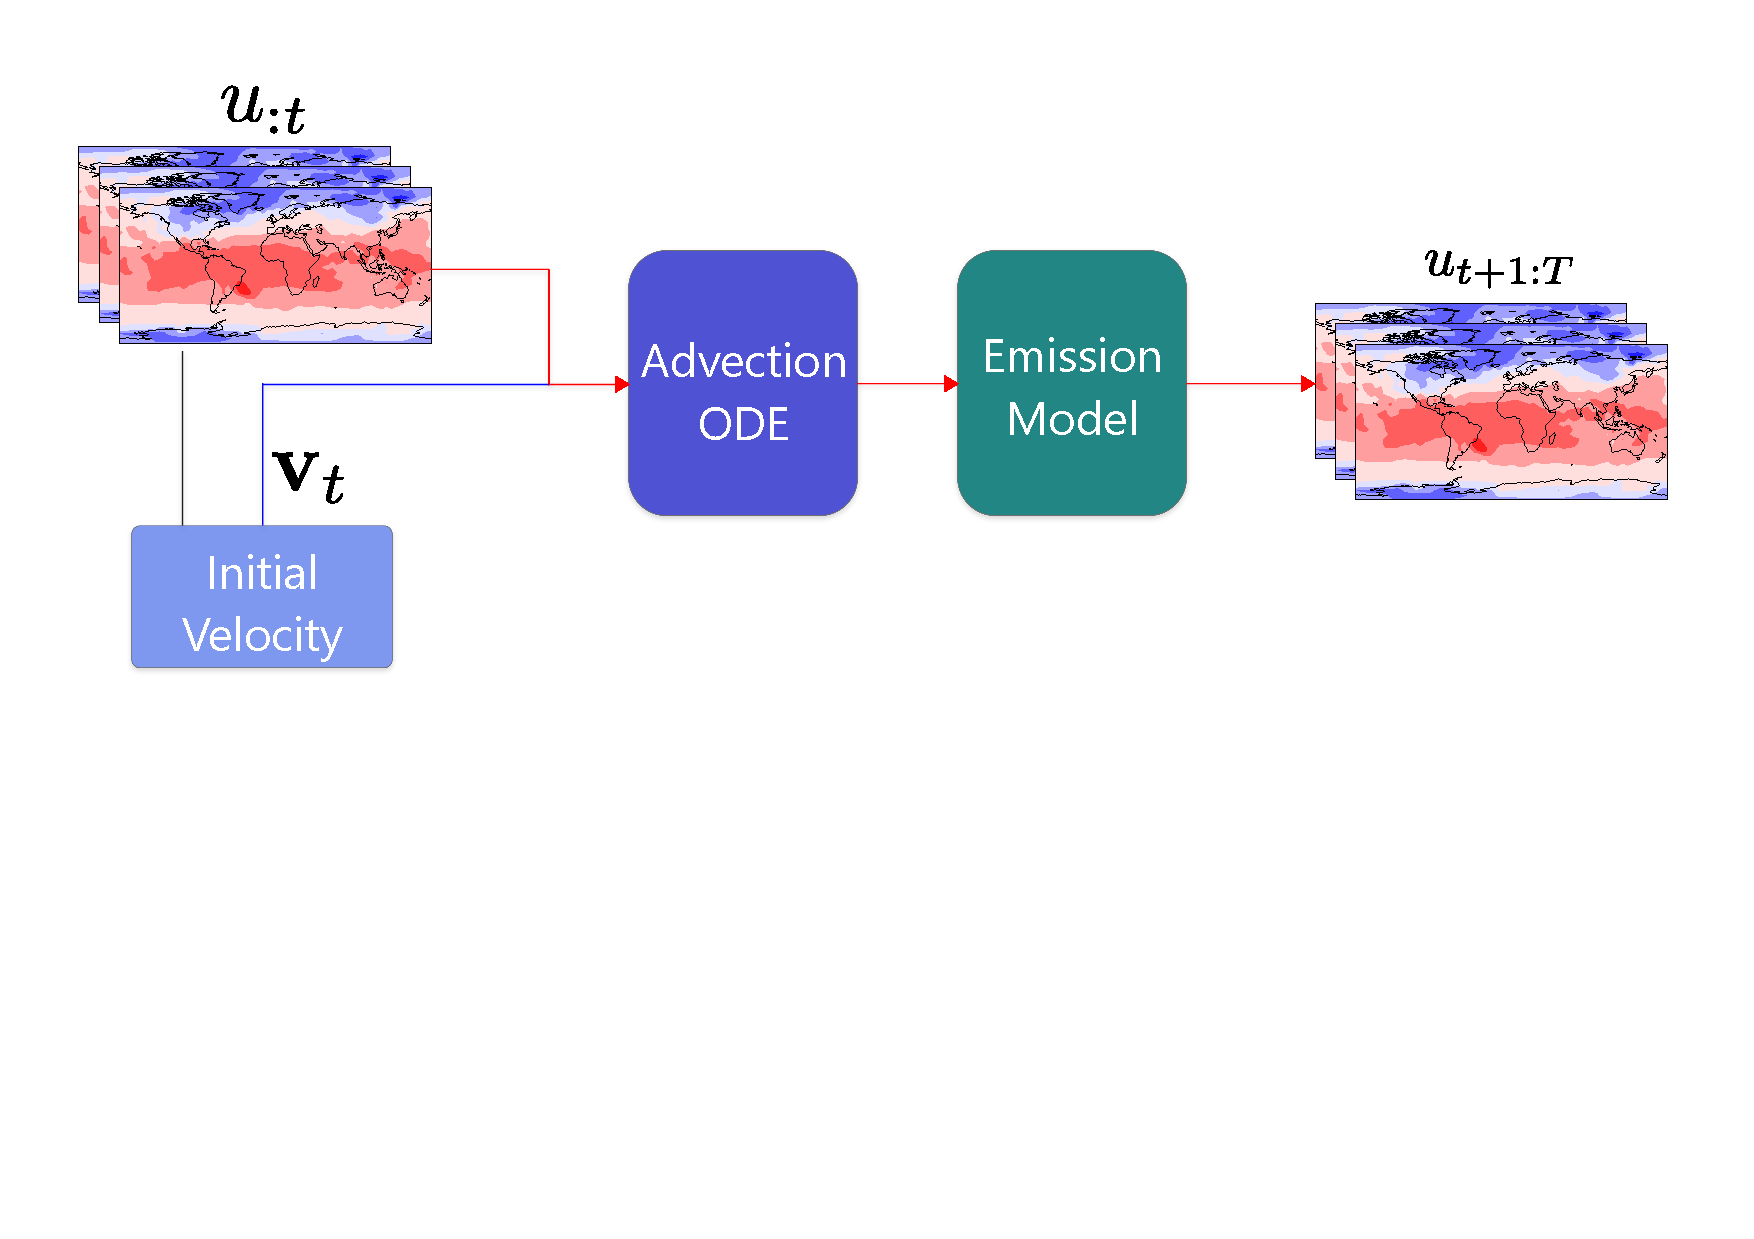
\includegraphics[width=0.5\textwidth]{ClimODE.pdf}
            % 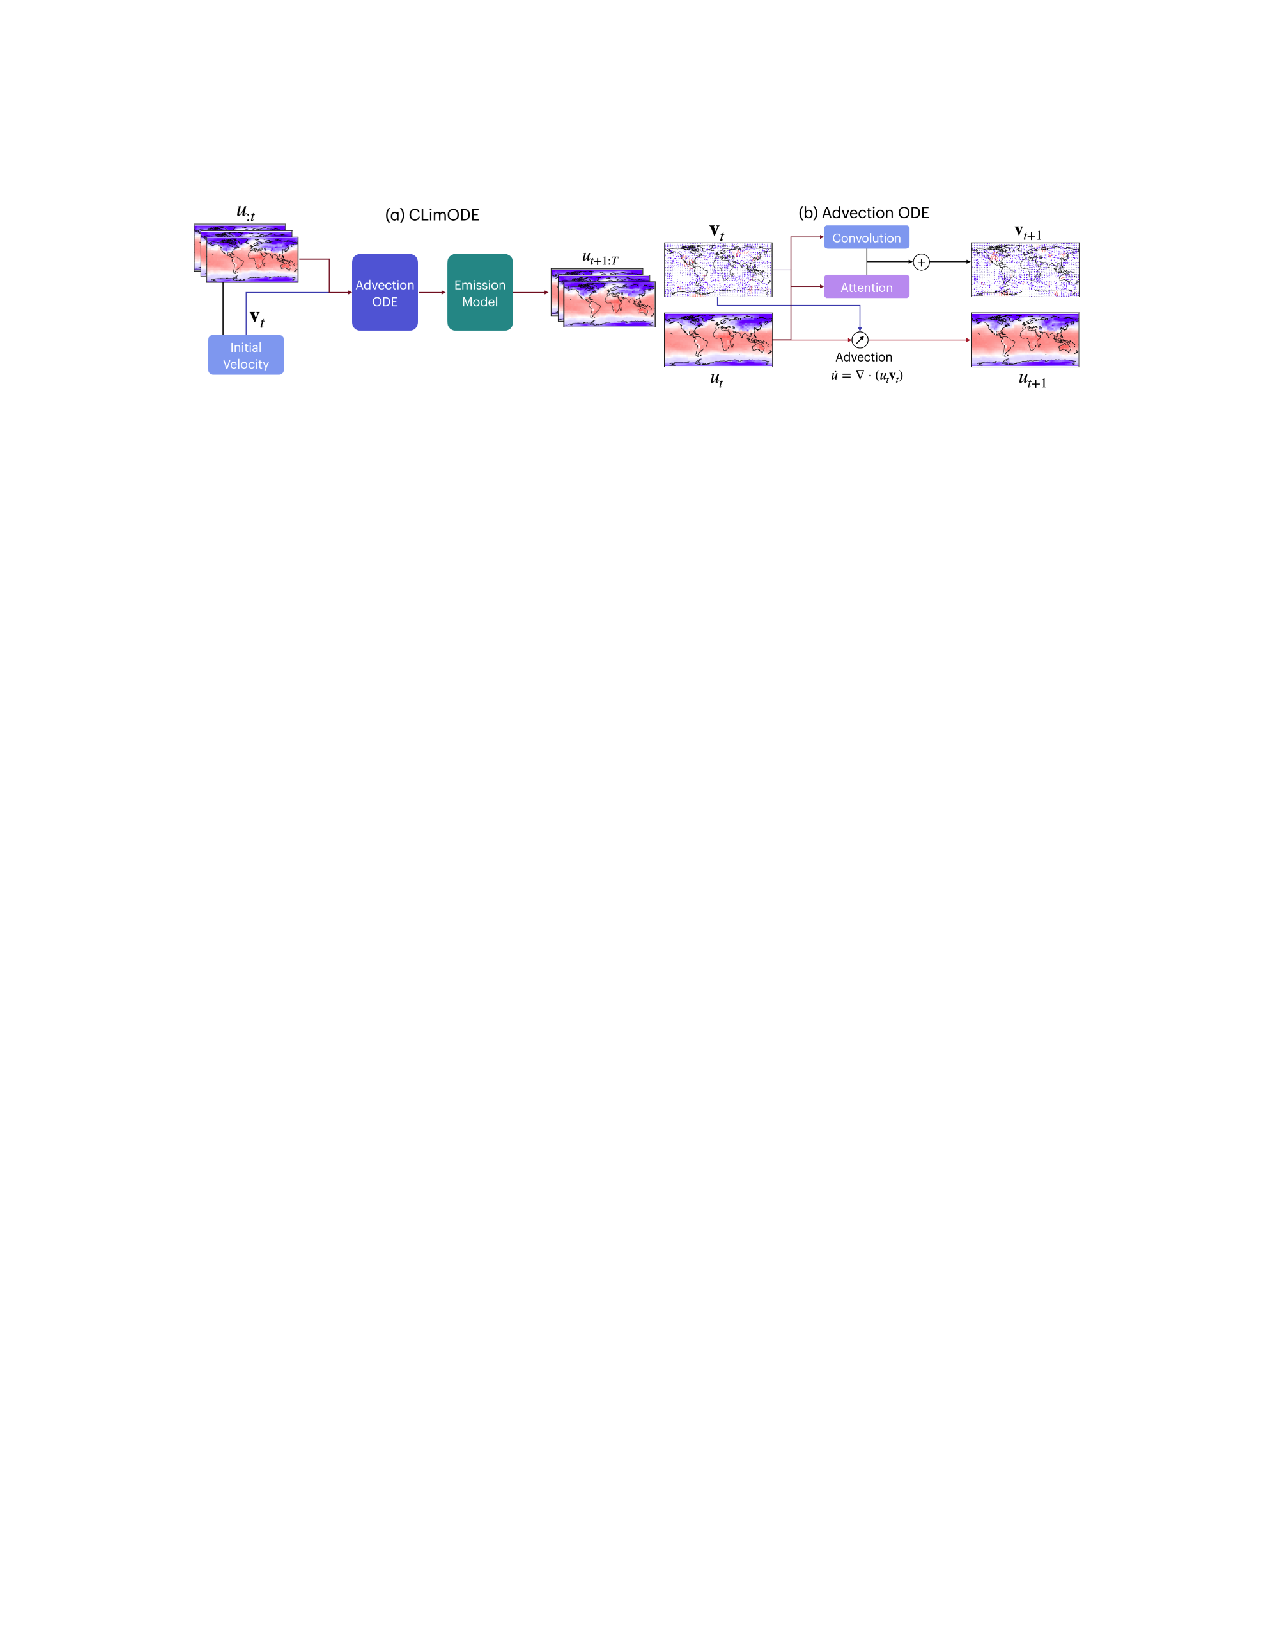
\includegraphics[width=\textwidth]{pipeline.pdf}
        \end{center}
        \vspace{-0.5em}
        %
        \textbf{\color{blue}Initial Velocity Inference:}
        \vspace{-0.5em}
        \begin{equation*}
            \hat{\mathbf{v}}_{k}(t) = \argmin_{\hat{\mathbf{v}}_{k}(t)} \left\{ \big\Vert \tilde{\dot{u}}_k(t) + \mathbf{v}_{k}(t) \cdot \tilde{\nabla}u_k(t) + u_k(t) \tilde{\nabla} \cdot \mathbf{v}_k(x,t) \big\Vert_2^2 + \alpha \big\Vert \mathbf{v}_k(t) \big\Vert \right\}
        \end{equation*}
        %
        \textbf{\color{blue}Flow Velocity:} % Modeling Local and Global Effects
        \vspace{-0.5em}
        \begin{equation*}
            \dot{\mathbf{v}}_k(x,t) = f_{\text{conv}} \left( \mathbf{u}(t), \nabla \mathbf{u}(t), \mathbf{v}(t), \psi \right) + \gamma f_{\text{att}} \left( \mathbf{u}(t), \nabla \mathbf{u}(t), \mathbf{v}(t), \psi \right) % f_{\theta}(\mathbf{u}(t), \nabla \mathbf{u}(t), \mathbf{v}(t), \psi) 
        \end{equation*}
        %
        \textbf{\color{blue}Advection ODE:} 
        \vspace{-0.5em}
        \begin{equation*}
            \begin{bmatrix}\mathbf{u}(t) \\ \mathbf{v}(t)\end{bmatrix} 
            % = \begin{bmatrix}\mathbf{u}(t_0) \\ \mathbf{v}(t_0)\end{bmatrix} + \int_{t_0}^{t} \begin{bmatrix}\dot{\mathbf{u}}(\tau) \\ \dot{\mathbf{v}}(\tau) \end{bmatrix}  \,d\tau 
            = \begin{bmatrix} \{u_k(t_0)\}_k \\ \{ \mathbf{v_k}(t_0) \}_k \end{bmatrix} + \int_{t_0}^{t} \begin{bmatrix} \{  - \nabla \cdot \left( u_k(\tau)  \mathbf{v}_k(\tau) \right) \}_k \\ \{ f_{\theta}(\mathbf{u}(\tau), \nabla \mathbf{u}(\tau), \mathbf{\tau}(t), \psi)_k  \}_k \end{bmatrix} \,d\tau
        \end{equation*}
        %
        \textbf{\color{blue}Emission Model:} 
        \vspace{-0.5em}
        \begin{equation*}
            u_{k}^{\mathrm{obs}}({\bf x},t)\sim{\cal N}\left(u_{k}({\bf x},t)+\mu_{k}({\bf x},t),\sigma_{k}^{2}({\bf x},t)\right), \ \mu_{k}({\bf x},t),\sigma_{k}({\bf x},t)=g_{k}\left({\bf u}({\bf x},t),\psi\right)
        \end{equation*}
        \vspace{-0.5em}
        %
        \textbf{\color{blue}Loss Function:} % Negative log-likelihood of the observations $\mathbf{y}_i \in \mathbb{R}^{K \times H \times W}$ at times $t_i$ :
        \vspace{-0.5em}
        \begin{equation*}
            \mathcal{L}_{\theta} = - \frac{1}{NKHW} \sum_{i=1}^{N} \left( \log \mathcal{N}\left(\mathbf{y}_{i}|\mathbf{u}(t_{i}) + \boldsymbol{\mu}(t_{i}), \text{diag}\ \boldsymbol{\sigma}^{2}(t_{i})\right) + \log \mathcal{N}_{+}\left(\boldsymbol{\sigma}(t_{i})|\boldsymbol{0},\lambda_{\sigma}^{2}I\right) \right)
        \end{equation*}
    }
    %
    \headerbox{\bf\color{blue} Experiments \& Results}{name=results,column=2,row=0,span=4}{
        % \begin{minipage}[t]{0.50\textwidth}
        %     \textbf{\color{blue}Synthetic Training Datasets:} 
        %     \vspace{-0.8em}
        %     \begin{center}
        %         \includegraphics[width=\textwidth]{images/syn_samples.pdf}
        %     \end{center}

        %     \vspace{0.1em}
        %     \textbf{\color{blue}Lighting Distribution of Real Datasets:} 
        %     \vspace{-0.2em}
        %     \begin{center}
        %         \includegraphics[width=0.95\textwidth]{images/real_lighting_dist.pdf}
        %     \end{center}
        % \end{minipage}\hfill
        % \begin{minipage}[t]{0.47\textwidth}
        %     \textbf{\color{blue}Results on DiLiGenT Benchmark~[2]:} 
        %     \vspace{-0.2em}
        %     \begin{center}
        %         \includegraphics[width=0.98\textwidth]{images/quant_diligent.pdf}
        %     \end{center}
        % \end{minipage}

        % \vspace{0.7em}
        % \textbf{\color{blue}Quantitative Results on {\sc Bunny} Rendered with $100$ MERL BRDFs:} \\
        % \vspace{-1.0em}
        % \begin{minipage}[t]{0.23\textwidth}
        %     \vspace{-9.5em}
        %     \begin{center}
        %         \includegraphics[width=0.48\textwidth]{images/MERL_directions.jpg}
        %         \includegraphics[width=0.48\textwidth]{images/bunny_normal.png}\\
        %         \vspace{-0.5em}
        %         \makebox[0.48\textwidth]{\scriptsize (a) Light source} 
        %         \makebox[0.48\textwidth]{\scriptsize (b) {\sc Bunny}} 
        %     \end{center}
        % \end{minipage}
        % \begin{minipage}[t]{0.76\textwidth}
        %     \begin{center}
        %         \includegraphics[width=\textwidth]{images/Bunny_100MERL.pdf}
        %     \end{center}
        % \end{minipage}

        % \textbf{\color{blue}Quantitaive Comparison on {\sc Harvest} in DiLiGenT Benchmark:} \\
        % \begin{center}
        %     \vspace{-0.6cm}
        %     \includegraphics[width=\textwidth]{images/qual_diligent_harvest.pdf}
        % \end{center}

        % \vspace{-0.8em}
        % \begin{minipage}[t]{0.72\textwidth}
        %     \textbf{\color{blue}Qualitative Results on Gourd\&Apple Dataset~[11] and Light Stage Data Gallery~[12]:} \\
        %     \vspace{-1.5em}
        %     \begin{center}
        %         \includegraphics[width=\textwidth]{images/qual_others.pdf}
        %     \end{center}
        % \end{minipage}
    }
    %
    \headerbox{\bf\color{blue} Critics}{name=critics,column=2,below=results,span=4}{
        
    }
    %
\end{poster}
\end{document}
